% vim: tw=80 noai
\documentclass[a4]{article}
%\usepackage[latin1]{inputenc}
\usepackage[utf8]{inputenc}
%\usepackage[T1]{fontenc}
\usepackage[brazil]{babel}
\usepackage{url}
\usepackage{graphicx}
\usepackage{listings}
\usepackage{verbatim}
\usepackage{subfigure}
\usepackage{multicol}
\usepackage{framed}

%\hyphenation{ab-stract}

%%%%%%%%%%%%%%%%%%%%%%%%%%%%%%%%%%%%%%%%%%%%%%%%%%%%
\def\lstlistingname{Listagem}

% Comandos
%\newcommand{\TODO}{\textbf{TODO:} }

\newcommand{\web}{\emph{web}}

\begin{document}

\begin{abstract}
% Kent Beck's four sentences for a good abstract:
%% the problem
%% why the problem is a problem
%% startling sentence
%% implication of the startling sentence

  Muitos sistemas não têm uma arquitetura bem documentada.
  Sem arquitetura bem documentada é difícil entender o sistema e planejar mudanças
  O uso de tecnicas de mineracao e algoritmos de clustering ajuda a construir uma visão arquitetural do sistema.
    Avaliamos algumas dessas técnicas
  Essas tecnicas revelam bla-bla-bla.
  

bli~\cite{Maqbool2007}

\textbf{Keywords:} 
aspect-oriented modeling,
reverse engineering,
software visualization.
\end{abstract}

% Introducao sobre recuperacao arquitetural (e trabalhos relacionados). 
% Clustering
%% Descricao das entidades, descricao de acoplamento, ...
%% Caracteristicas de software
% Algoritmo hierárquico aglomerativo e técnicas associadas
%% AHA - merges são finais
%% AHA - algoritmo guloso, otimização local
%% AHA - medidas monotonicamente relacionadas (
%% AHA - usa matriz de similaridade, que pode codificar qualquer critério
% Experimento
%% Sistemas avaliados
%%% Caracteristicas: densidade, similaridade media, desvio-padrao da simil.
%% Criterios de avaliacao (authoritative..., size, stability)
% Resultados experimentais e sua interpretacao
%% Threats to validity.
%%% As métricas são uma merda. O extractor funciona bem?
%% Avaliacao quantitativa
%% Avaliacao qualitativa
% Discussao
%% O que significa esse particionamento? Pra que serve?

%%
\section{Introdução} \label{intro}

O conjunto de decisões mais significativas de um software formam 
arquitetura do software. Essas decisões devem ser tomadas cedo no processo
de desenvolvimento do software, pois elas afetam um grande número de decisões
que devem ser tomadas ao longo do desenvolvimento.

As decisões arquiteturais são motivadas pelos requisitos do sistema e dizem
respeito a uma parte de seus \emph{stakeholders}. É comum dividir a
arquitetura em diversas visões, cada uma delas contemplando um subconjunto
dos requisitos e dos \emph{stakeholders}. A visão lógica, por exemplo,
é destinada principalmente aos \emph{designers} e programadores e trata de
requisitos como a facilidade de manutenção e de compreensão do \emph{software}.
[cite 4+1]

O campo de pesquisa denominado recuperação de arquitetura de software tem como
objetivo extrair aspectos da arquitetura de um sistema a partir de artefatos
criados durante seu desenvolvimento. A maioria dos trabalhos na
área se concentra na recuperação de uma visão lógica da arquitetura de um
sistema a partir da análise de seu código-fonte.

Uma boa porção desses trabalhos emprega algoritmos de agrupamento
(\emph{clustering}) para identificar grupos de entidades de código-fonte
(tipicamente funções e classes). Um bom agrupamento deve
fornecer a desenvolvedores uma visão geral do sistema e deve revelar atributos
de qualidade do software como reusabilidade, manutenibilidade e facilidade de
compreensão.

%% trabalhos relacionados?? Anquetil e Lethbridge, Maqbool e Babri.



%%%%
%
\section{Recuperação de arquitetura a partir de código-fonte} \label{sec:recovery}

A recuperação da arquitetura de um sistema a partir de seu código-fonte pode
ser dividida em duas etapas: a extração do design do sistema e a abstração
desse design para uma descrição arquitetural.

%Para extrair o design, usamos a ferramenta Design Wizard, que faz análise
%estática de programas escritos em Java. 

O design extraído do código-fonte é
descrito por um grafo onde os vértices representam as classes do sistema
e as arestas representam dependências entre as classes. 
A etapa de abstração consiste na aplicação de algoritmos de agrupamento sobre
as classes do design. O resultado é uma decomposição do sistema em módulos
arquiteturais concebidos de forma que cada módulo contém classes similares.

%Essa dependência
%ocorre em diversas situações --- por exemplo, quando uma classe possui uma
%referência para um objeto de outra classe, ou quando um de seus métodos chama
%algum método de outra classe.

É necessário, portanto, quantificar a similaridade entre cada par de classes
de um sistema. A métrica de similaridade pode considerar diversas 
características de classes, tais como identificadores e comentários a elas
associados, relações de dependências entre classes ou o histórico de 
modificações.
%os nomes das classes e comentários a elas associados, a identidade dos
%desenvolvedores que modificaram a classe ou a quantidade de modificações.
%Neste trabalho, a métrica de similaridade é definida a partir
%das relações de dependência entre as classes. 
%Cada classe é representada
%como o conjunto de classes das quais ela depende. 

Existe uma literatura vasta sobre algoritmos de agrupamento. Neste trabalho
avaliaremos o algoritmo de agrupamento hierárquico aglomerativo.

%%%%%%%%%%%%%%%%%%%%%%%%%%%%%%%%%%%%%%%%%%%%%%%%%%%%%%%%%%%%%%%%%%%%%%%%%%%%%%
%%%%%%%%%%%%%%%%%%%%%%%%%%%%%%%%%%%%%%%%%%%%%%%%%%%%%%%%%%%%%%%%%%%%%%%%%%%%%%
%%%%%%%%%%%%%%%%%%%%%%%%%%%%%%%%%%%%%%%%%%%%%%%%%%%%%%%%%%%%%%%%%%%%%%%%%%%%%%
%%%%%%%%%%%%%%%%%%%%%%%%%%%%%%%%%%%%%%%%%%%%%%%%%%%%%%%%%%%%%%%%%%%%%%%%%%%%%%
%%%%%%%%%%%%%%%%%%%%%%%%%%%%%%%%%%%%%%%%%%%%%%%%%%%%%%%%%%%%%%%%%%%%%%%%%%%%%%
%%%%%%%%%%%%%%%%%%%%%%%%%%%%%%%%%%%%%%%%%%%%%%%%%%%%%%%%%%%%%%%%%%%%%%%%%%%%%%

\subsection{Algoritmo hierárquico algomerativo} \label{sec:aha}

O algoritmo hierárquico aglomerativo produz, a partir de um conjunto
de entidades e de uma métrica de similaridade entre entidades, uma hierarquia
de grupos (\emph{clusters}), como mostra a Figura \ref{fig:dendograma}. 
Cada grupo da hierarquia contém dois grupos menores.
A hierarquia pode ser
representada por uma árvore (chamada de dendograma) cujas folhas
são grupos unitários (que contêm apenas uma entidade) e cuja raiz
representa um grupo que contém, transitivamente, todas as entidades do
sistema.

%Nessa hierarquia, dois módulos podem ser agrupados em um
%módulo maior.
%Nessa hierarquia, cada módulo contém outros dois módulos, com
%exceção dos módulos unitários, que contém uma classe.

%%%%%%%%%%%%%%%%%%%%%%%%%%%%%%%%%%%%%%%%%%%%%%%%%%%%%%%%%%%%%%%%%%%%%%
\begin{figure}[ht] \label{fig:dendograma}
\begin{centering}
  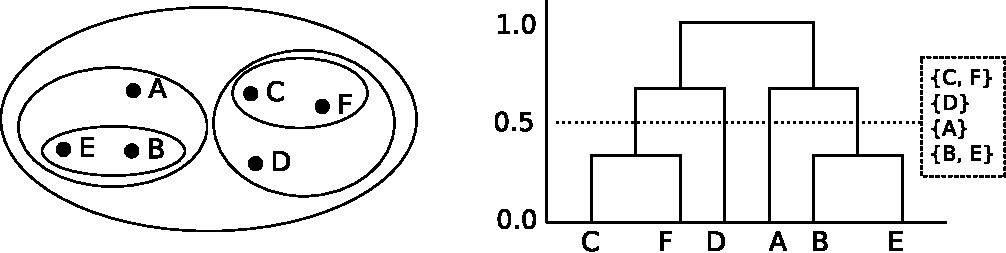
\includegraphics[width=1.0\textwidth]{fig_dendograma}
  \caption{Duas representações de um dendograma e particionamento produzido
  por um corte na altura 0.5 ou 50\%}
\end{centering}
\end{figure}
%%%%%%%%%%%%%%%%%%%%%%%%%%%%%%%%%%%%%%%%%%%%%%%%%%%%%%%%%%%%%%%%%%%%%%

O algoritmo considera inicialmente cada entidade como um grupo unitário e, a 
cada passo, agrupa os dois grupos mais similares até que reste apenas um
grupo. A Figura \ref{fig:algoritmo} apresenta o algoritmo em pseudo-código.

%%%%%%%%%%%%%%%%%%%%%%%%%%%%%%%%%%%%%%%%%%%%%%%%%%%%%%%%%%%%%%%%%%%%%%
\begin{figure}[ht] \label{fig:algoritmo}
\begin{centering}
  \begin{verbatim}
  raizes = {}
  para cada entidade C: raizes = adicione {C} a raizes
  enquanto #raizes > 2
    Escolha A, B em raizes tal que similaridade(A, B) é máxima
    adicione {A, B} a raizes
    remova A de raizes
    remova B de raizes

  dendograma = raizes
  \end{verbatim}
  \caption{Pseudo-código do algoritmo hierárquico aglomerativo}
\end{centering}
\end{figure}
%%%%%%%%%%%%%%%%%%%%%%%%%%%%%%%%%%%%%%%%%%%%%%%%%%%%%%%%%%%%%%%%%%%%%%

A similaridade entre dois grupos pode ser definida de diversas maneiras,
dentre as quais podem-se citar \emph{single linkage} e \emph{complete
linkage}.
No \emph{single linkage}, a similaridade entre dois grupos é definida como
a maior similaridade entre dois elementos, um de cada grupo.
No \emph{complete linkage}, considera-se a menor similaridade.
A Figura \ref{fig:linkage} ilustra os dois conceitos.

%%%%%%%%%%%%%%%%%%%%%%%%%%%%%%%%%%%%%%%%%%%%%%%%%%%%%%%%%%%%%%%%%%%%%%
\begin{figure}[ht] \label{fig:linkage}
\begin{centering}
  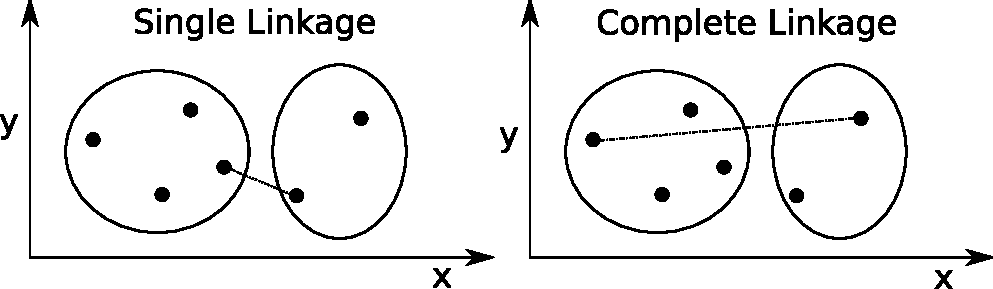
\includegraphics[width=1.0\textwidth]{fig_linkage}
  \caption{Duas métricas de similaridade entre grupos: 
    \emph{single linkage} e \emph{complete linkage}. Nesta ilustração,
    a similaridade entre dois pontos é definida como o inverso da distância
    entre eles no plano cartesiano.}
\end{centering}
\end{figure}
%%%%%%%%%%%%%%%%%%%%%%%%%%%%%%%%%%%%%%%%%%%%%%%%%%%%%%%%%%%%%%%%%%%%%%

O resultado do algoritmo hierárquico é uma decomposição aninhada do sistema.
Para obter um particionamento do sistema --- na qual cada grupo contém
apenas entidades --- é preciso cortar o dendograma em alguma altura.
Um corte na altura 0 produz grupos unitários, enquanto um
corte na altura 1 (100\%) produz um grupo que contém todas as entidades.
A Figura \ref{fig:dendograma} ilustra um corte na altura 0.5 ou 50\%.

\subsubsection{Características}

O algoritmo hierárquico aglomerativo é determinístico: ele sempre produz o
mesmo dendograma quando recebe as mesmas entradas. Seu tempo de execução é
de $O(n^3)$ e o espaço ocupado é $O(n^2)$, onde $n$ é o número de entidades.
Essa complexidade é considerada alta e o algoritmo torna-se inviável quando
submetido a um grande volume de dados.

O algoritmo procura maximizar a similaridade entre
entidades dentro de um grupo, mas faz isso de maneira local. Não há 
garantias de que a decomposição final seja ótima em relação à similaridade
dentro de um grupo. 

Os agrupamentos realizados pelo algoritmo são definitivos: dois grupos 
unidos jamais serão separados. Por essa razão as primeiras iterações
são especialmente importantes. Um grupo mal formado no início é propagado
até o final do algoritmo.

% O algoritmo assume muito pouco sobre os dados --- ele apenas exige 

%
%
%As primeiras iterações do algoritmo são especialmente importantes, pois
%
%merges são finais.
%algoritmo guloso, otimização local.
%medidas monotonicamente relacionadas.
%usa matriz de similaridade, que pode codificar qualquer critério.
%complexidade alta
%determinístico

%%%%%%%%%%%%%%%%%%%%%%%%%%%%%%%%%%%%%%%%%%%%%%%%%%%%%%%%%%%%
% 
% A técnica aqui apresentada 
% 
% Modelo de design OO: grafo
% 
% Clustering: coloca no mesmo grupo entidades similares
% 
% Como definir a similaridade entre entidades?
%   Parâmetros formais.
%   Parâmetros não-formais. (Anquetil)
% 
% Algoritmo ha. (Anquetil, Maqbool)
%   Explicação.
%   Similaridade entre clusters.
%   Critério de parada, ponto de corte.
% 
% Características do algoritmo ha.
%   merges são finais.
%   algoritmo guloso, otimização local.
%   medidas monotonicamente relacionadas.
%   usa matriz de similaridade, que pode codificar qualquer critério.
% 
% Técnicas.
%   k-NN: k-nearest neighbors.
%   SNN: shared nearest neighbors.
%   aplicar distância à matriz de similaridade para obter outra.
% 

%\section{Avaliação}



%%%
%\input{metodologia.tex}

%\input{estudoDeCaso.tex}
%
%\input{conclusoes.tex}




\bibliographystyle{alpha}
\bibliography{evolucao2008}

\end{document}
